\section{TP1: Bling Bling}
\subsection{Objectif}
Dans ce TP nous allons commencer par faire clignoter une LED, puis nous utilserons la led RGB poru afficher une couleur précise, finalement nous ferons un compte à rebour avec l'afficheur 7 segments et l'afficheur 4 fois 7 segments.

\subsection{Matériel}
\begin{itemize}
	\item Un ordinateur
	\item Un arduino Uno R3
	\item Une LED simple
	\item Une LED RGB
	\item Un afficheur 7 segments
	\item Un afficheur 4 fois 7 segments
	\item Une résistance de 220$\Omega$
\end{itemize}

\subsection{LED clignotante}
Dans cette manipulation nous allons faire clignotter une LED en la branchant au port 13 de l'arduino. Ce port correspond également à la LED inclue dans l'arduino, nous pourrions donc même ici nous passer de la breadboard. Nous mettons bien sur aussi une résistance de 220$\Omega$ en série avec la LED, mais nous aurions aussi pu utiliser la résistance \textit{pullup}.
\lstinputlisting[language=C]{Code/TP1/TP1.1/TP1.1.ino}
\begin{figure}[H]
	\centering
	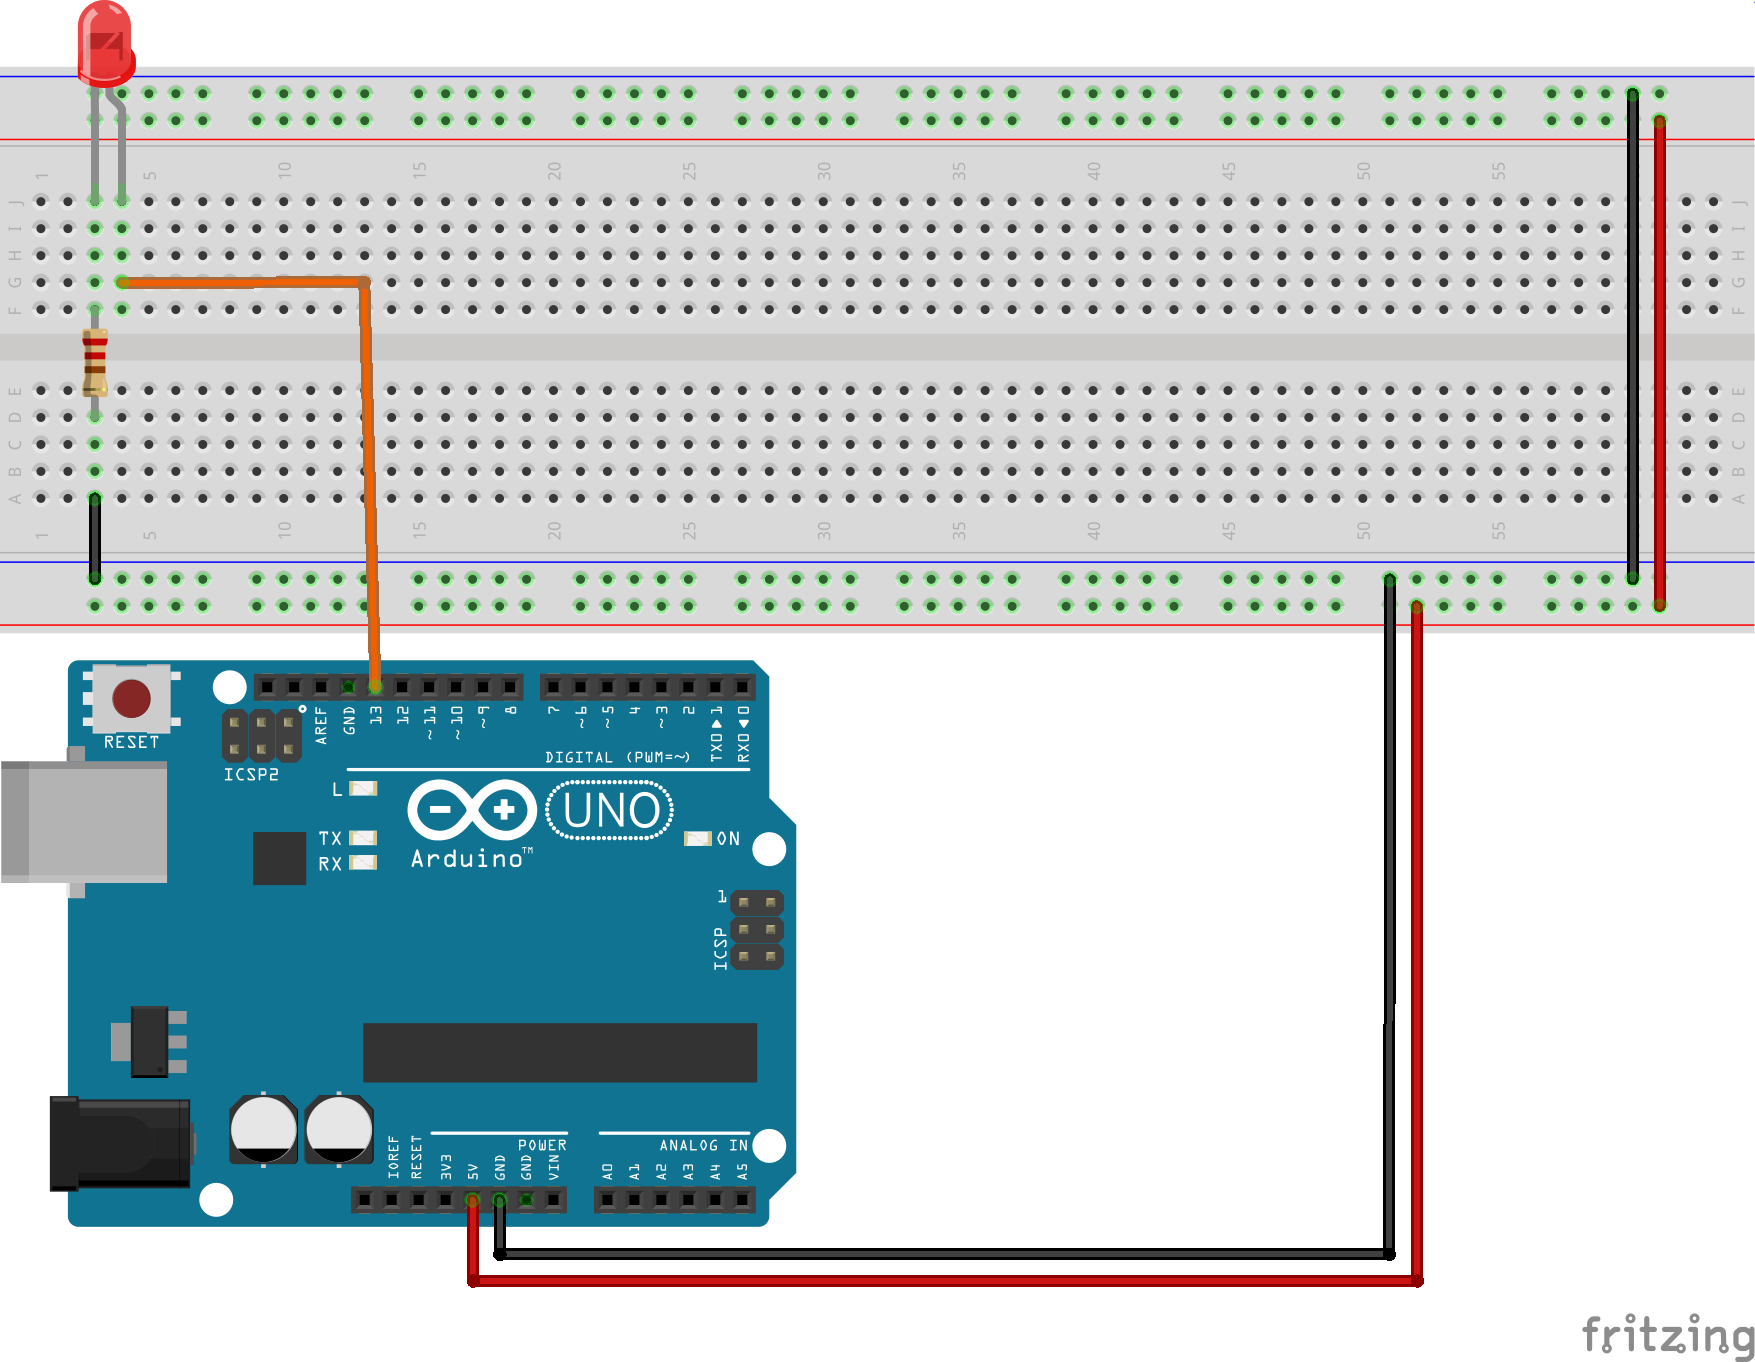
\includegraphics[height=6cm]{img/TP1-1.png}
	\caption{\label{TP1.1}LED clignotante}
\end{figure}
%TODO LED

\subsection{LED RGB}
Dans cette manipulaton nous allons controller la couleur d'une LED RGB qui est en faite composée de 3 LED, une rouge, une verte et une bleu. Nous relions donc les pattes correspondantes aux couleurs à notre arduino et la patte correspondant à la cathode commune au +VCC via une résistance\@. Le code correspondant à une LED RGB à annode commune est aussi inclu. Nous utilisons les ports analogiques et non digitaux pour pouvoir controler l'intensité de chaque couleur et ainsi allumer la LED de la couleur souhaitée.
\lstinputlisting[language=C]{Code/TP1/TP1.2/TP1.2.ino}
\begin{figure}[H]
	\centering
	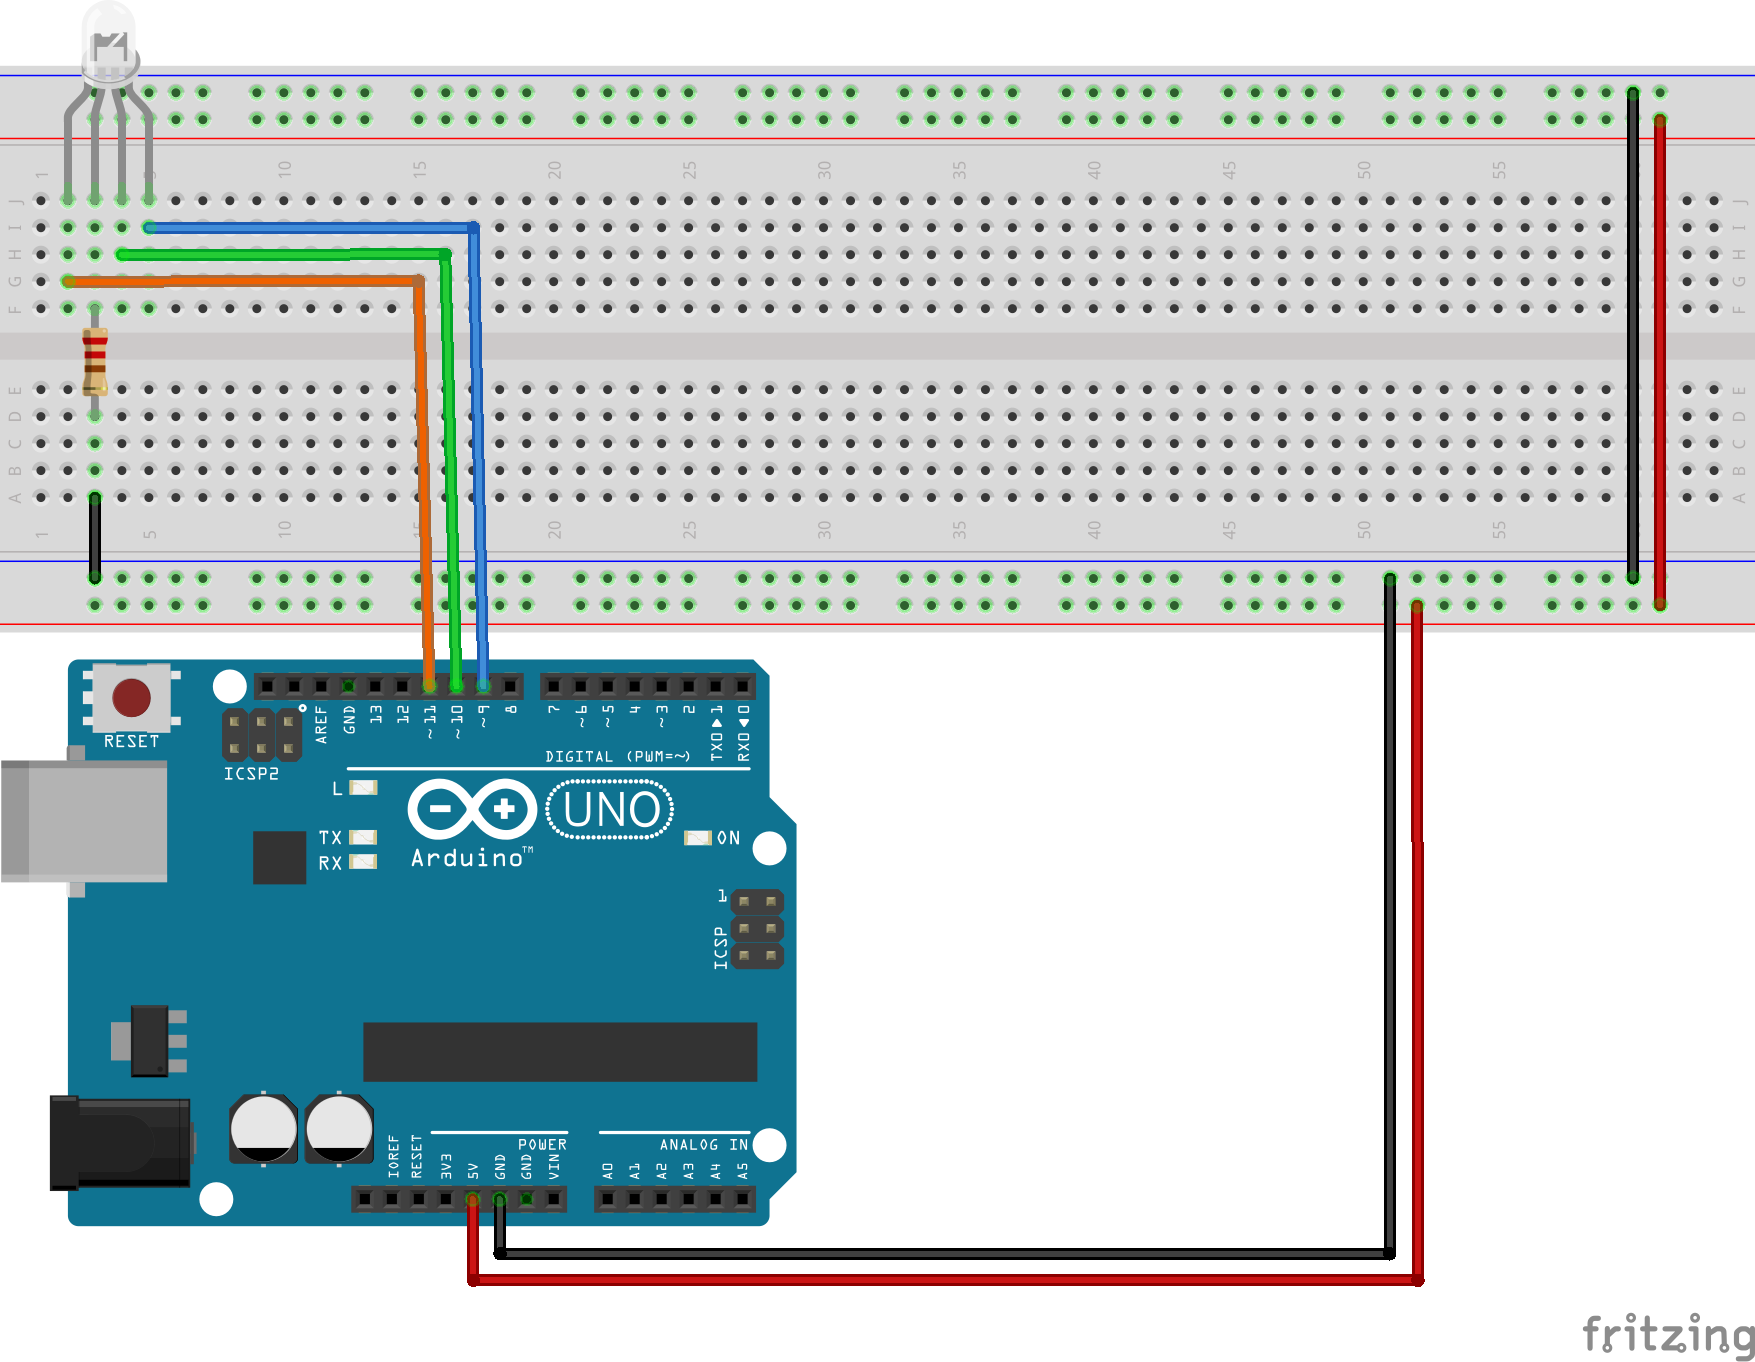
\includegraphics[height=6cm]{img/TP1-2.png}
	\caption{\label{TP1.2}LED RGB}
\end{figure}
%TODO LED RGB

\subsection{Afficheur 7 segments simple}
Dans cette manipulation nous allons connecter un afficheur 7 segments à un notre arduino pour lui faire afficher un compte à rebour allant de 9 à 0. Alternativement nous aurions pu lui faire aire un compte à rebour alant de F (16 en hexadécimal) à 0.
\lstinputlisting[language=C]{Code/TP1/TP1.3/TP1.3.ino}
\begin{figure}[H]
	\centering
	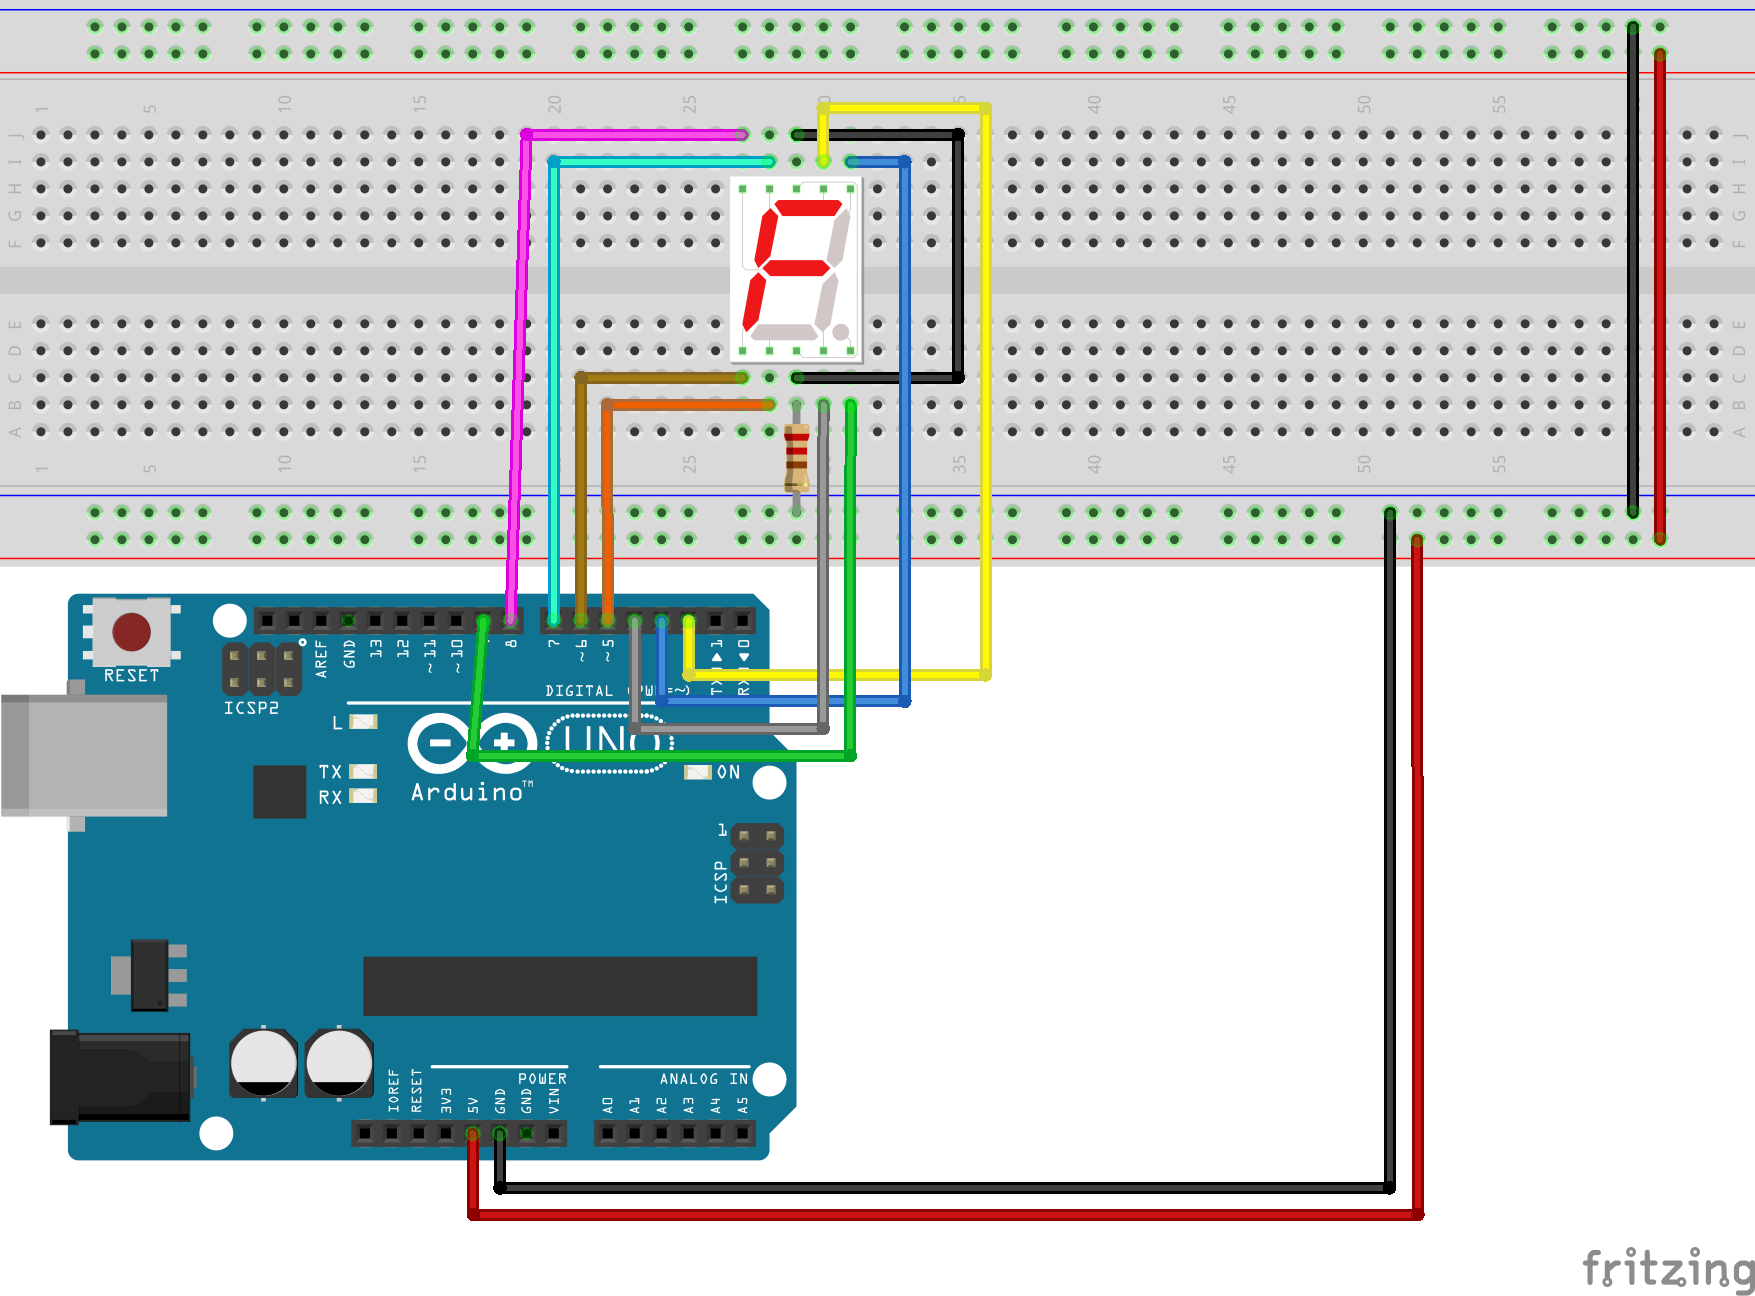
\includegraphics[height=6cm]{img/TP1-3.png}
	\caption{\label{TP1.3}Afficheur 7 segments}
\end{figure}
%TODO 7 Segments

\subsection{Afficheur 7 segments quadruple}
\lstinputlisting[language=C]{Code/TP1/TP1.4/TP1.4.ino}
\begin{figure}[H]
	\centering
	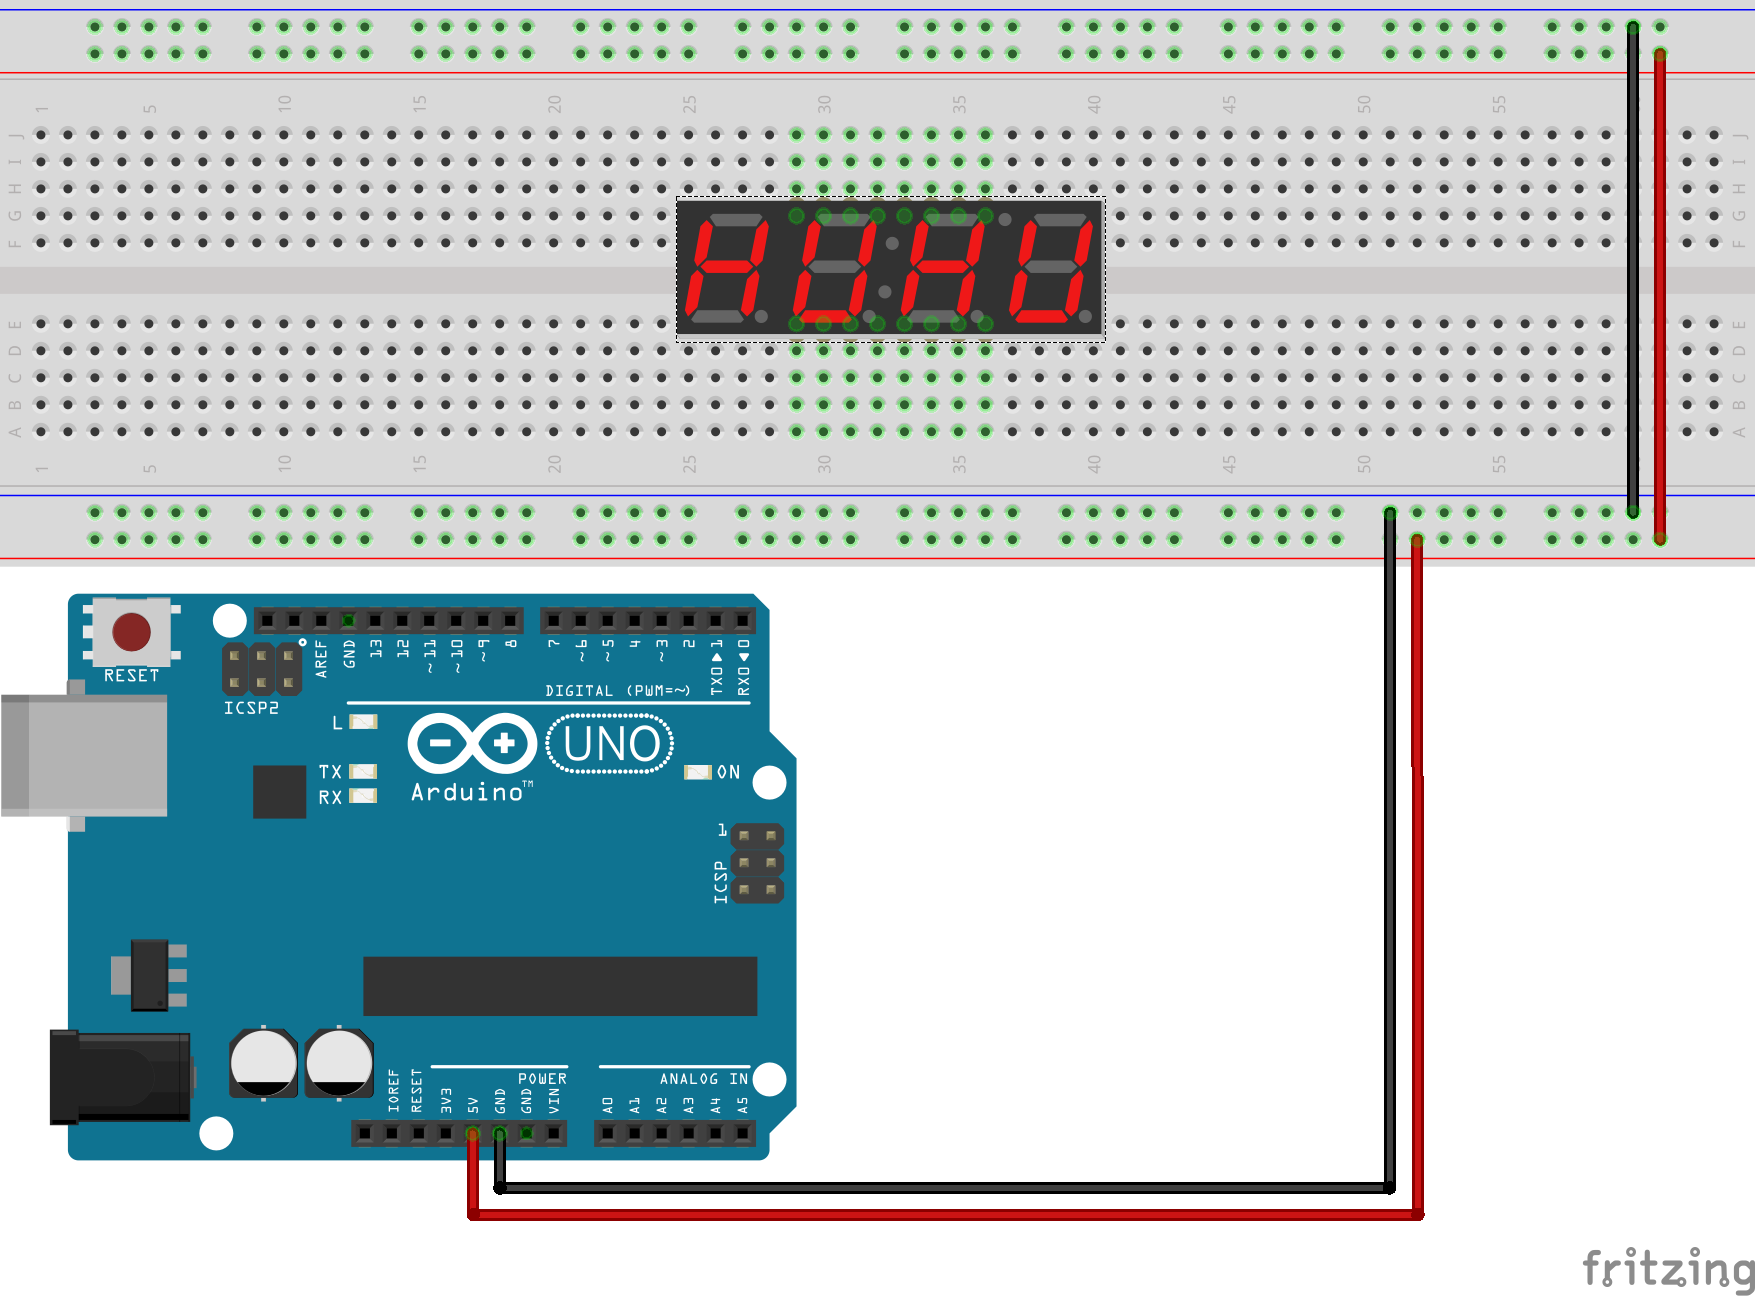
\includegraphics[height=6cm]{img/TP1-4.png}
	\caption{\label{TP1.4}Afficheur 7 segments quadruple}
\end{figure}
%TODO 7 Secgment quadruple
